\chapter{Presentation guidelines}
\label{chap:guidelines}
\selectlanguage{english}
You have downloaded the LaTeX AMU custom class for Aix-Marseille University doctoral theses. Some elements must be used:
\\


\begin{figure}[h!tbp]
	%\vspace{0.5cm}
	\centering
	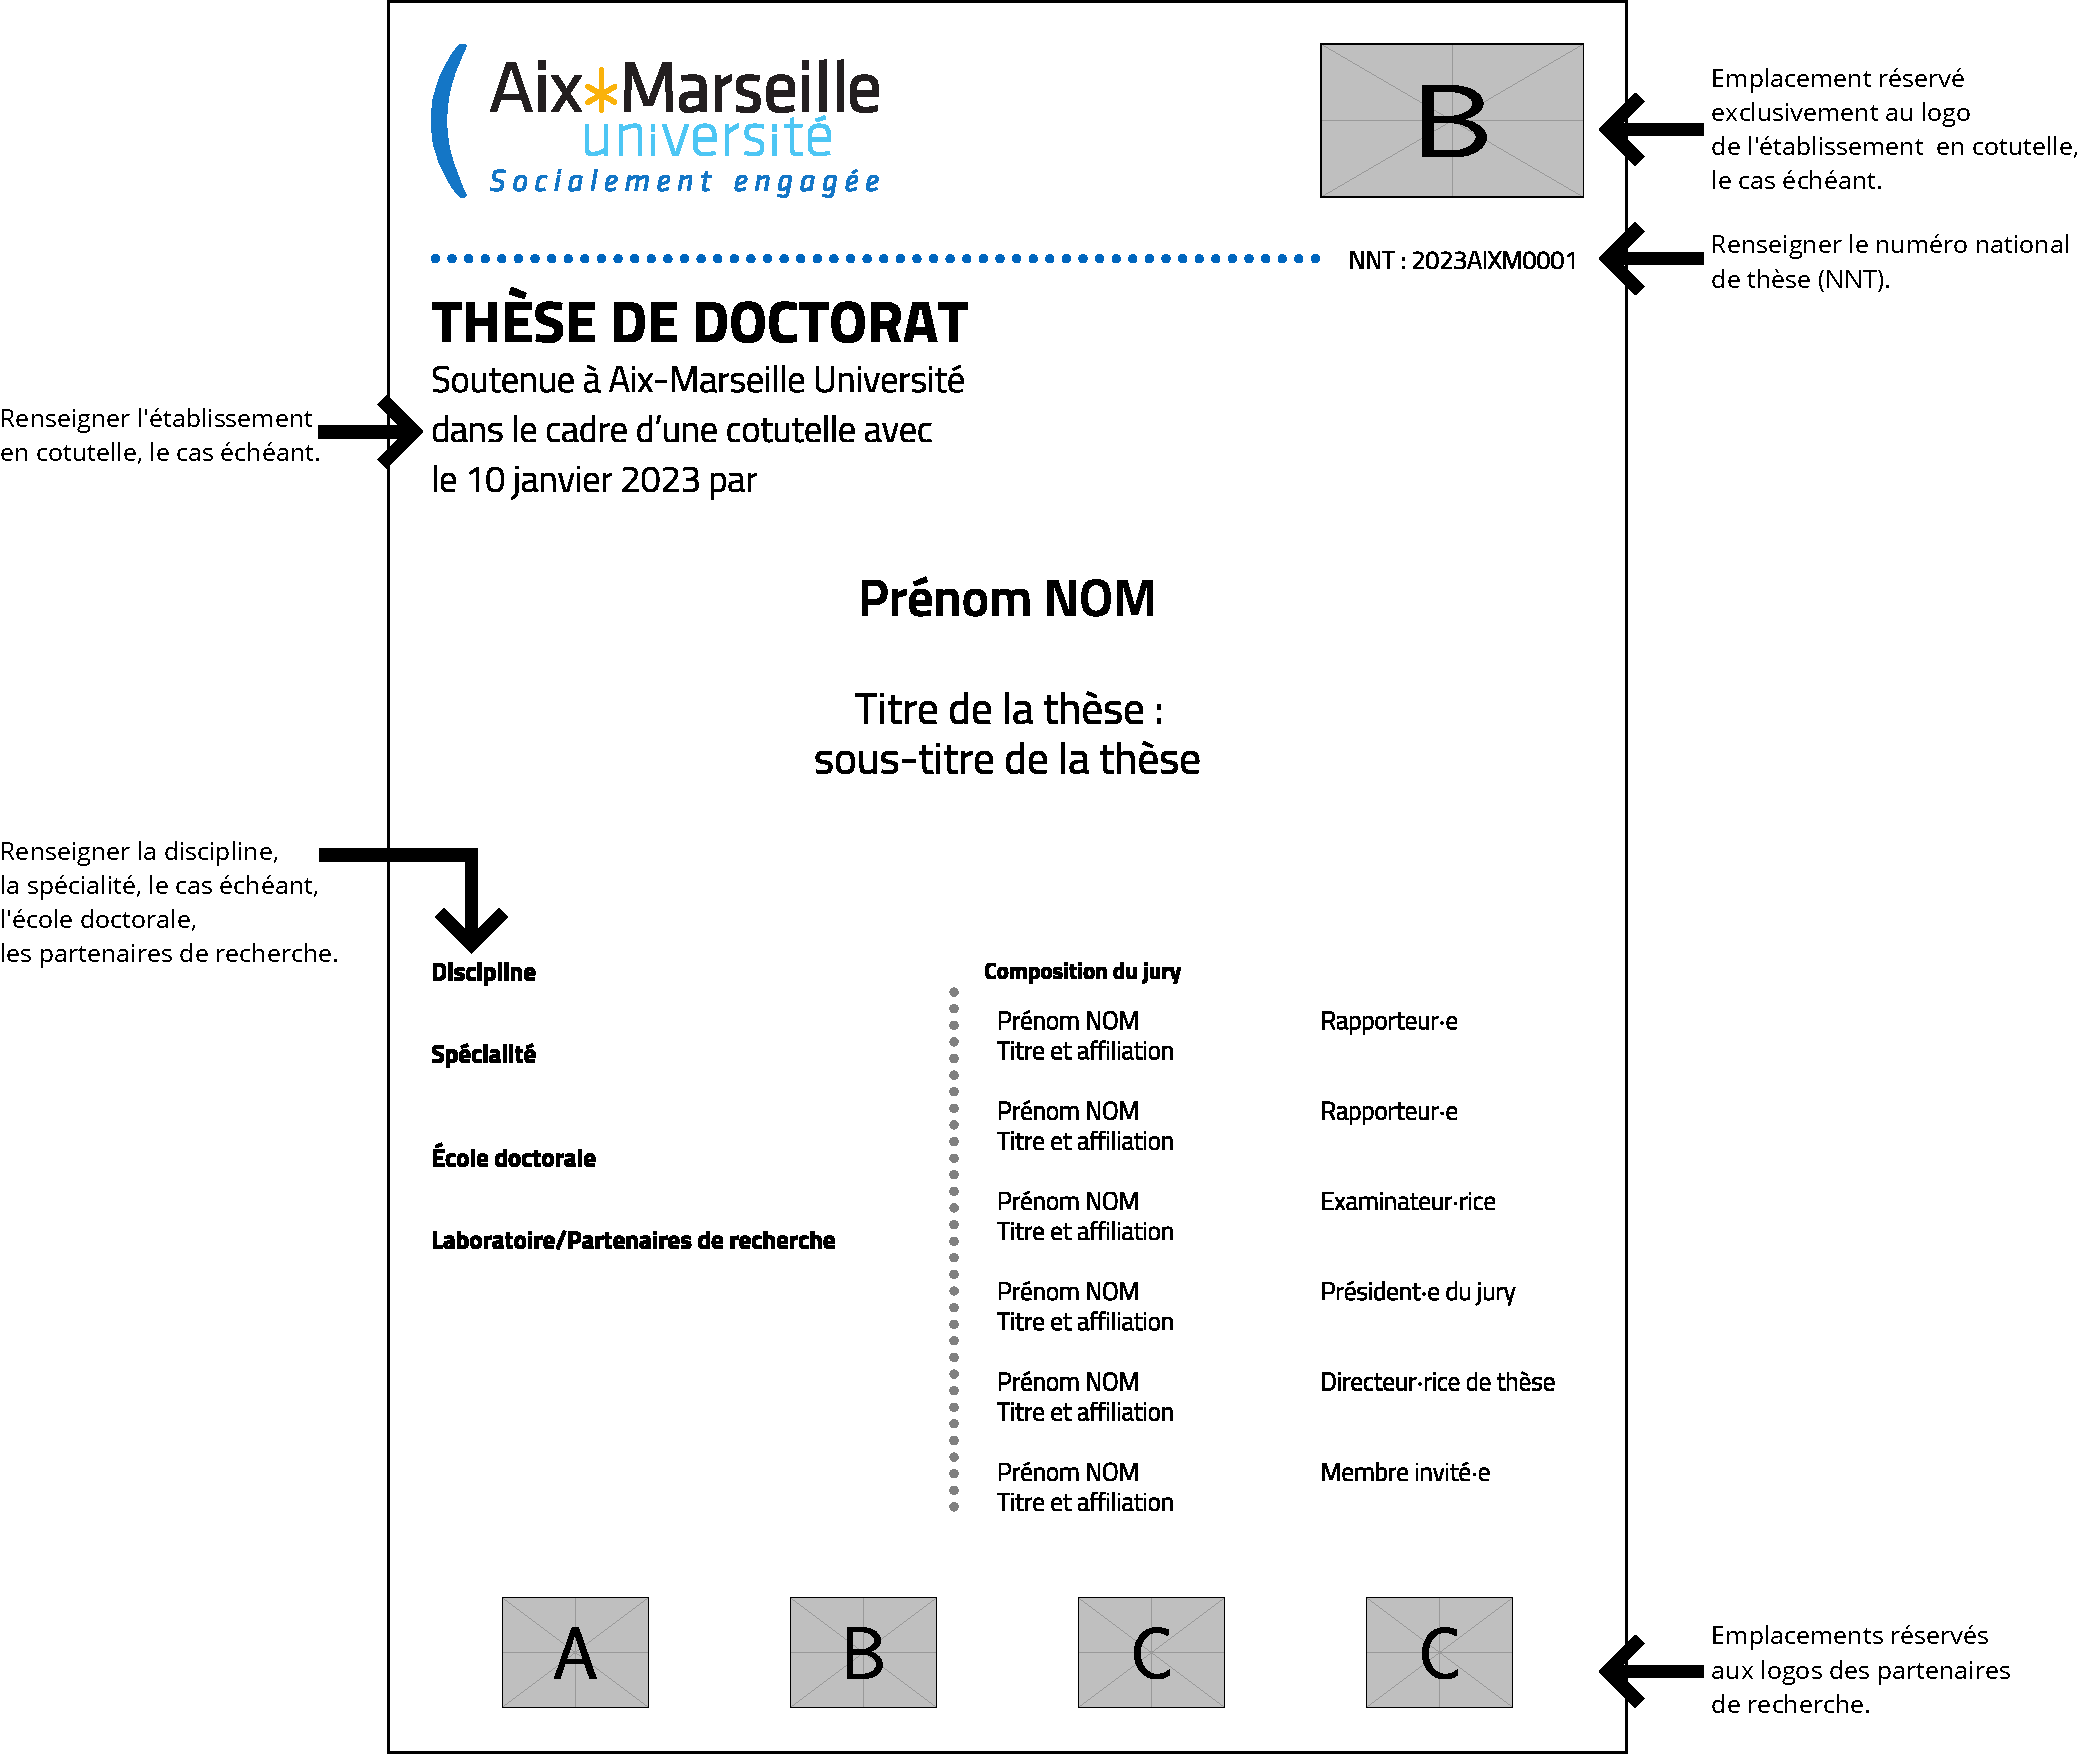
\includegraphics[width=0.8\textwidth]{titre.pdf}
\end{figure}

\begin{enumerate}
    \item The title page of AMU’s thesis: it is written in French with the Titillium font, provided with the LaTeX AMU template in TTF and TFM formats, according to AMU’s graphic charter.
    \item In the case of international cotutelle, the logo of the partner institution must appear at the top right of the title page;
	\item The composition of the jury, the doctoral school, the discipline and the specialty (if applicable) must be in accordance with the ADUM application form for the thesis defense;
	\item The national thesis number (NNT) must be displayed on the title page;
	\item Where appropriate, logos of partner institutions or research units can be added to the bottom of the title page;
	\item The \nameref{chap:affidavit} page: according to the language used for writing your thesis, choose the French or English version, then complete, date and sign it;
	\item The \nameref{chap:publications} page made during the course of your thesis project ;
	\item \nameref{chap:resume} in French and \nameref{chap:abstract} in English pages: each summary must not exceed 4,000 characters.\\
\end{enumerate}

Depending on your needs, you can add the following elements: summary and/or table of contents, list of figures, list of tables, list of acronyms, glossary, index, nomenclature...
For the body of your thesis, if your doctoral school does not give you more specific instructions, you can use the styles established in this template or your own styles following these recommendations:
\begin{itemize}
	\item Neutral font : It is recommended to use a standard serif font for text and a standard sans-serif font for titles;
	\item Geometry : paper=a4, fontsize=12pt, DIV=12;
	\item Single-line spacing;
	\item Justified text.\\
\end{itemize}

\begin{figure}[h!tbp]
	%\vspace{0.5cm}
	\centering
	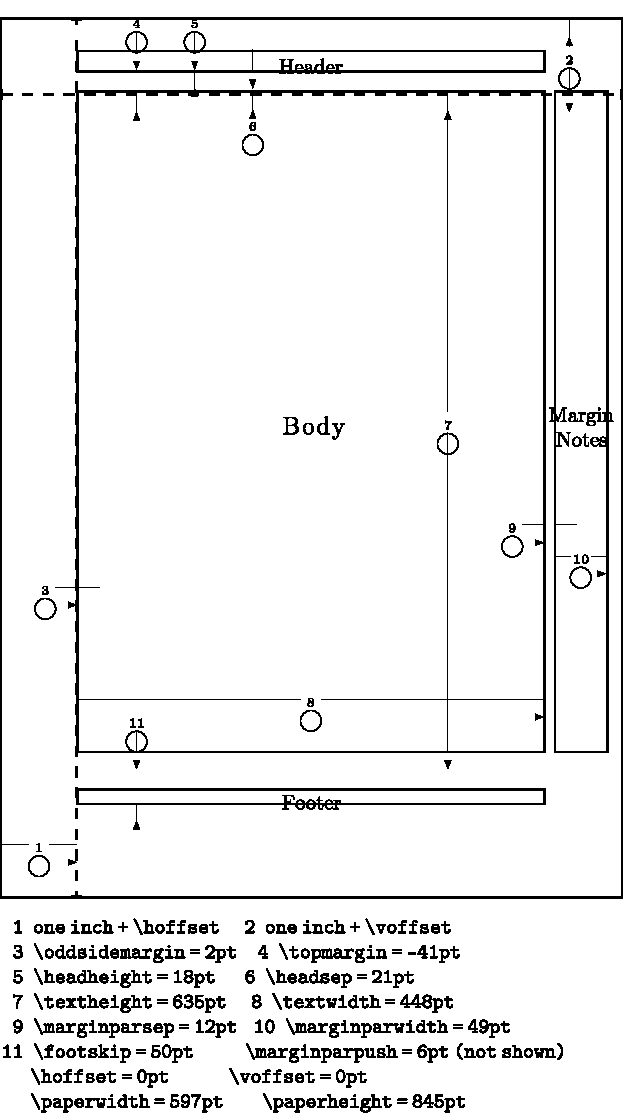
\includegraphics[width=0.3\textwidth]{geometry.pdf}
\end{figure}

Your thesis must be submitted online in PDF 1.5 minimum version format on \href{https://www.adum.fr/}{adum.fr}.

\selectlanguage{french}
